\documentclass[norsk,a4paper,12pt]{article}
\usepackage[utf8]{inputenc}
\usepackage{graphicx} %for å inkludere grafikk
\usepackage{verbatim} %for å inkludere filer med tegn LaTeX ikke liker
\usepackage{tabularx}
\usepackage{booktabs}
\usepackage{amsmath}
\usepackage{float}
\usepackage{color}
\usepackage{listings}
\usepackage{hyperref}
\usepackage{amsmath}
\usepackage{tikz}

\lstset{language=c++}
\lstset{basicstyle=\small}
\lstset{backgroundcolor=\color{white}}
\lstset{frame=single}
\lstset{stringstyle=\ttfamily}
\lstset{keywordstyle=\color{red}\bfseries}
\lstset{commentstyle=\itshape\color{blue}}
\lstset{showspaces=false}
\lstset{showstringspaces=false}
\lstset{showtabs=false}
\lstset{breaklines}
\lstset{postbreak=\raisebox{0ex}[0ex][0ex]{\ensuremath{\color{red}\hookrightarrow\space}}}
\usepackage{titlesec}

\setcounter{secnumdepth}{4}
\usetikzlibrary{through,calc,er,positioning}

\titleformat{\paragraph}
{\normalfont\normalsize\bfseries}{\theparagraph}{1em}{}
\titlespacing*{\paragraph}
{0pt}{3.25ex plus 1ex minus .2ex}{1.5ex plus .2ex}


\title{FYS4411 - Computational Physics II\\\vspace{2mm} \Large{Project 2}}
\author{\large Dorthea Gjestvang\\ Even Marius Nordhagen}
\date\today
\begin{document}

\maketitle

\begin{itemize}
\item Github repository containing programs and results: \\\url{https://github.com/evenmn/FYS4411/tree/master/Project%202}
\end{itemize}

\begin{abstract}
Abstract
\par 

\end{abstract}

\newpage

\tableofcontents

\newpage

\section{Introduction} \label{sec:Introduction}


\section{Theory} \label{sec:Theory}
\subsection{Presentation of potential} \label{sec:Presentation_of_potential}
In this project, we simulate a system of $P$ electrons trapped in a harmonic oscillator potential, with a Hamiltonian given by

\begin{equation}
\label{eq:Hamiltonian}
\hat{H} = \sum_{i=1}^{P} (-\frac{1}{2} \nabla_i^2 + \frac{1}{2} \omega^2 r_i ^2) + \sum_{i<j} \frac{1}{r_{ij}} 
\end{equation}

where $\omega$ is the harmonic oscillaor potential and  $r_i = \sqrt{x_i^2 + y_i^2}$ is the position of electron $i$. The term $\frac{1}{r_{ij}}$ is the interacting term, where $r_{ij} = |r_i - r_j|$ is the distance between a given pair of interacting electrons. Natural units have been used, such that $\hbar = c = m_e = e = 1$.

Since electrons are fermions, we need an antisymmetric wavefunction under exchange of two coordinates, and we need to take the Pauli principle into account. A Slater determinant is therefore needed for multiple fermions to ensure that the total wavefunction is antisymmetric. In this project we will study particles in the ground state only, and according to the Pauli principle we can in this case study a maximum of two particles with spin $s=\pm 1/2$. The slater determinant for two particles read
\begin{equation}
\Psi_T=
\begin{vmatrix}
\Phi_1(\boldsymbol{r}_1) & \Phi_2(\boldsymbol{r}_1)\\
\Phi_1(\boldsymbol{r}_2) & \Phi_2(\boldsymbol{r}_2)
\end{vmatrix}
=\Phi_1(\boldsymbol{r}_1)\Phi_2(\boldsymbol{r}_2)-\Phi_2(\boldsymbol{r}_1)\Phi_1(\boldsymbol{r}_2)
\end{equation}
where $\Phi_i(\boldsymbol{r})$ is the single particle wave function (SPF) of state $i$. This contains a spatial part and a spin part, and we assume that it can be splitted up such that the spin part takes the antisymmetry property and does not affect the energy. Therefore we only need a symmetric spatial part to calculate the energies.

\subsection{Solving this with machine learning}
Usually, when solving a system of particles as the one described in the previous system, we would need an anzats for the wave function, where we use our physical intuition to create the form of a wave function with different variational parameters, and then let it be up to the computer to find the optimal parameters through a minimization method. However, this method is only as good as the physical intuition; if the form of the wave function is unrealistic, the results will be the same, and there is no guarantee that we have actually found a ground state energy.
\par 
\vspace{3mm}
This challenge can be solved by using machine learning. There are several different types of machine learning systems, and the one we will present and utilize in this project has the ability to learn a probability distribution. This is perfect for quantum mechanical problems, as we know from quantum mechanics the wave function $\Psi$ is nothing more than a probability denisty, giving that $\Psi^2$ is a probability distribution that says something about where a given particle most probabliy can be found. As we are solely interested in the energy of the two-fermion system, and not the exact wave function, the fact that the machine learning program does not explicitly give the wave function is therefore of no consequence.

\subsubsection{Machine learning}
With the goal of solving the quantum mechanical system presented in section \ref{sec:Presentation_of_potential} in mind, we should start by explaining what machine learning is. Machine learning is the idea that a computer can be trained to learn to yield certaint outputs, without directly being told exactly what to give. Examples on this is pattern recognizion, where the computer first is shown for example pictures of wolves and huskies. After training the computer on pictures where the computer sees huskies and wolves and is told the correct answer, it should after a sufficiently long training period, be able to recognize huskies and wolves by itself. 
\par 
\vspace{3mm}
The example described above is what we call supervised learning, where the correct output answer is known during the training program. A machine learning program could also be unsupervised, where the correct answer is unknown, or based on reinforcement learning, where the the program learns by conducting trial-and-error experiments. 
\par 
\vspace{3mm}

\subsubsection{Neural network}

 This sound amazing, and maybe even impossible. Therefore the question now is: how to program computers to learn, just like humans? The answer is, fittingly, that we should make the program run like the the human brain by implementing what is called a neural network. Inspired by neurons in the human brain, a neural network is a programmed network of variables, called nodes, that comminucate in a given manner. Each node preforms a simple process: based on the input it receives, and how that input is weighted, it decides wheter or not to fire. The mathematical model of an example of a neural node was presented by McCulloch and Pitts in 1943 \cite{Marsland}, shown in figure \ref{fig:neuron}, where the input is mared $x_i$, the weights deciding how much the input should count is $W_i$, and the output from the node based on $x_i$ and $W_i$ is called h. 
 
 \begin{figure} [H]
 	\centering
 	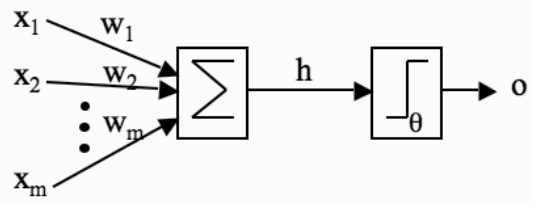
\includegraphics[scale=0.6]{plots/neuron.png}
 	\caption{McCullochs and Pitts' model of neutrons visualized. Image reproduced from \cite{Marsland} }
 	\label{fig:neuron}
 \end{figure}

The neutrons are arranged in layers in the neural network, one visible layer that receives the input, and up to several hidden layers. The layers are arranged such that the output values from the visible nodes is the input values of the visible nodes. The nodes can also have bias values, that shift the output value $h$ with a ceirtan number, and the nodes in different layers can be connected in different ways.  An example of a neural network with two layers is shown in figure \ref{fig:neural_network}.

 \begin{figure} [H]
	\centering
	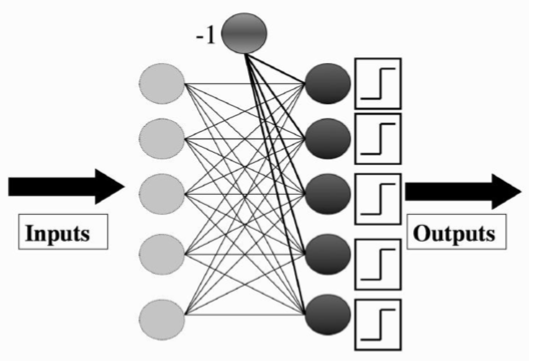
\includegraphics[scale=0.5]{plots/neural_network.png}
	\caption{An example of a neural network with one visible and one hidden layer of nodes, and with bias $-1$ on the hidden nodes. Image reproduced from \cite{Marsland} }
	\label{fig:neural_network}
\end{figure}

The idea behind machine learning is that the weights $W_i$, that decides how much a node puts emphazis on a given input, can be changed, and thus change the system's response to the same input. We will explain with the example from earlier, with huskies and the wolves: first, the program are shown pictures of wolves and huskies, and it is told the correct answer. The weights $W_i$ are then updated such that when a husky is shown, the output "husky" is generated, and the same for wolves. After a sufficiently long training period, the program's weights are optimalized for recognizing wolves and huskies. When shown a picture, the program should then by itself be able to determine wheter it is a wolf or a husky that it sees. 

\subsubsection{Restricted Boltzmann Machines}
There are plenty of ways to put together a neural network, as one can modify the number of nodes and layers, the bias, and also which nodes that are allowed to communicated. In this project, we will be using the so-called Restricted Boltzmann Machine (RBM). It is a two-layer network. The reason why it is named "restrictive" is that there are no connections between nodes in the same layer, but every node in the previous layer is connected to all the nodes in the next layer. The RBM can learn to draw samples from a probability distribution, which is just what we want in our project. In addition, we want to use a Gaussian-Binary RBM, where the hidden nodes have binary values, while the positions of the particles can take continous values, as they are, in fact, positions. 


\subsection{Energy calculation}



\subsection{Onebody density}

\subsection{Scaling}

\subsection{Error estimation}

\section{Method}

\subsection{Variational Monte Carlo}
\subsection{Metropolis Algorithm}
\subsubsection{Brute force}
\subsubsection{Importance sampling}
\subsubsection{Gibbs sampling}

\subsection{Minimalization method}
\subsubsection{Gradient decent}

\section{Code}
\subsection{Structure}
\subsection{Implementation}

\section{Results} \label{sec:Results}

\section{Discussion} \label{sec:Discussion}

\section{Conclusion} \label{sec:Conclusion}

\newpage

\section{Appendix A} \label{sec:appendix_A}

\newpage
\section{References}

\textcolor{red}{INCLUDE ONLY THOSE REFERENSES WE USE}

\begingroup
\renewcommand{\section}[2]{}
\begin{thebibliography}{}
	\bibitem{MHJ15}
	Morten Hjorth-Jensen.
	Computational Physics 2: Variational Monte Carlo methods, Lecture Notes Spring 2018.
	Department of Physics, University of Oslo,
	(2018).
	\bibitem{DuBois}
	J. L. DuBois and H. R. Glyde, H. R., \emph{Bose-Einstein condensation in trapped bosons: A variational Monte Carlo analysis}, Phys. Rev. A \textbf{63}, 023602 (2001).
	\bibitem{Nilsen}
	J. K. Nilsen,  J. Mur-Petit, M. Guilleumas, M. Hjorth-Jensen, and A. Polls, \emph{Vortices in atomic Bose-Einstein condensates in the large-gas-parameter region}, Phys. Rev. A \textbf{71}, 053610, (2005).
	\bibitem{Dalfovo}
	F. Dalfovo, S. Stringari, \emph{Bosons in anisotropic traps: ground state and vortices} Phys. Rev. A \textbf{53}, 2477, (1996).
	\bibitem{JE2016}
	J. Emspak, \emph{States of Matter: Bose-Einstein Condensate}, LiveScience, (2016).
	\url{https://www.livescience.com/54667-bose-einstein-condensate.html}
	Downloaded March 15th 2018.
	\bibitem{SP}
	S. Perkowitz \emph{Bose-Einstein condensate} Encyclopaedia Britannica 
	\url{https://www.britannica.com/science/Bose-Einstein-condensate}
	Downloaded March 15th 2018.
	\bibitem{Anderson}
	M. H. Anderson, J. R. Ensher, M. R. Matthews, C. E. Wieman, E. A. Cornell, \emph{Observation of Bose-Einstein Condensation in a Dilute Atomic Vapor}, Science \textbf{269}, (1995).
	\bibitem{JKNilsen}
	J. K. Nilsen \emph{Bose-Einstein condensation in trapped bosons: A quantum Monte Carlo analysis}, Master thesis 2004, Department of Physics, University of Oslo, (2004). 
	\bibitem{Gross}
	E. P. Gross, \emph{Structure of a quantized vortex in boson systems}, Il Nuovo Cimento, \textbf{20} (3): 454–457, (1961).
	\bibitem{Pitaevskii}
	L. P. Pitaevskii, \emph{Vortex lines in an imperfect Bose gas}, Sov. Phys. JETP. \textbf{13} (2): 451–454, (1961).
	\bibitem{Marsland}
	S. Marsland, \emph{Machine Learning: An algorithmic Perspective, Second edition} (2015)
	\bibitem{Nordhagen}
	E. M. Nordhagen and D.Gjestvang \emph{Computational Physics II: Project 1} (2018)
	
	
\end{thebibliography}
\endgroup

\end{document}
